\section{Скалярное произведение}

\begin{definition}
    Евклидово пространство --- это векторное пространство $V$ над $\mathbb{R}$
    вместе с билинейным отображением $\langle\cdot,\cdot\rangle \colon V \times V  \to \mathbb{R}$,
    такое что
    \[
    \begin{aligned}
        &\forall v \in V, \ v \ne 0 \quad \langle v,v\rangle > 0, \\
        &\forall v, w \in V \quad \langle v, w\rangle = \langle w, v\rangle.
    \end{aligned}
    \]
\end{definition}

\begin{examplelist}
        \item $V = \mathbb{R}^n$
            \[
            \langle
            \begin{pmatrix} v_1 \\ v_2 \\ \vdots \\ v_n \end{pmatrix},
            \begin{pmatrix} w_1 \\ w_2 \\ \vdots \\ w_n \end{pmatrix}
            \rangle
            := \sum_{i=1}^{n} v_i w_i
            \]
        \item $V = C([0,1])$
            \[
            \langle f, g\rangle := \int_0^1 f(x)\, g(x)\, dx
            \]
            Пусть $f \neq 0$, тогда
            \[
            \langle f, f\rangle = \int_0^1 f(x)^2\, dx > 0
            \]
\end{examplelist}


\begin{definition}
    Ортогональность:
    $v, w \in V \qquad v \perp w$, если $\langle v,w\rangle = 0$
\end{definition}

\begin{definition}
    Норма вектора:
    $v \in V \qquad \lVert v \rVert \coloneqq \sqrt{\langle v, v \rangle}$
\end{definition}

\begin{definition}
    Нормирование вектора:
    $v \neq 0 \qquad \hat{v} := \frac{v}{\|v\|}$

    \[
        \left\lVert \frac{v}{\|v\|} \right\rVert
        = \|v\| \cdot
        \frac{1}{\|v\|} = 1
    \]
\end{definition}


\begin{definition}
    Базис $e_1, e_2, \dots , e_n$ евклидова пространства $V$ называется \emph{ортогональным}, если $\langle e_i, e_j\rangle = 0$ при
    $i \neq j.\\$
    Такой базис называется \emph{ортонормированным}, если дополнительно $\|e_i\| = 1 \ \ \forall i = 1, \dots ,n.$
\end{definition}

\begin{example}
    Стардартный базис в $\mathbb{R}^n$:
    \[
    \|\mathbf{e}_i\| = \sqrt{0^2 + \cdots + 0^2 + 1^2 + 0^2 + \cdots + 0^2} = 1.
    \]
\end{example}

\begin{stmt}
    Ортогональное преобразование не меняет ортогональности

  \begin{center}
    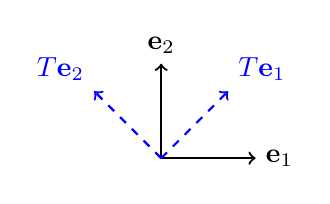
\begin{tikzpicture}
      \draw[->, thick] (0,0) -- (1.2,0) node[right] {$\mathbf{e}_1$};
      \draw[->, thick] (0,0) -- (0,1.2) node[above] {$\mathbf{e}_2$};
      \draw[->, thick, dashed, blue] (0,0) -- (0.85,0.85) node[above right] {$T\mathbf{e}_1$};
      \draw[->, thick, dashed, blue] (0,0) -- (-0.85,0.85) node[above left]  {$T\mathbf{e}_2$};
    \end{tikzpicture}
  \end{center}
\end{stmt}


\begin{example}

$L^2([0,\pi])$

Скалярное произведение:
\[
\langle f,g\rangle = \int_0^\pi fg\,dx
\]

Система функций $\bigl\{\cos nx,\ \sin mx\bigr\}_{\substack{n \geq 0 \\ m \geq 1}}$
--- разложение по базису -- ряд Фурье


$\int_0^\pi \cos x \sin x \, dx = \frac{1}{2} \int_0^\pi d\sin^2 x =
\frac{1}{2} \sin^2 x \Big|_0^\pi = 0 $
\par

\emph{(lection version, idk)}

% $\int_0^\pi \cos x \sin x \, dx = \frac{1}{2} \int_0^\pi \sin 2x \, dx =
% -\frac{1}{4} \cos 2x \Big|_0^\pi = -\frac{1}{4} (1 - 1) = 0$
\end{example}


\begin{stmt}
    Ортогональный набор $e_1, \dots, e_n$, где $e_i \neq 0$, линейно независим.
    \begin{proof}
        Пусть $\exists\, \mathbf{\lambda}_1, \dots, \mathbf{\lambda}_n \in \mathbb{R} : \sum_{i=1}^{n} \mathbf{\lambda}_i e_i = 0$
        \begin{align*}
            \forall j = 1,\dots,n \quad
            0 &= \Bigl\langle \sum_{i=1}^{n}\mathbf{\lambda}_i e_i,\, e_j\Bigr\rangle
               = \sum_{i=1}^{n} \mathbf{\lambda}_i \langle e_i, e_j\rangle \\[4pt]
              &= \mathbf{\lambda}_j \underbrace{\langle e_j, e_j\rangle}_{>\,0}
               \implies \mathbf{\lambda}_j = 0
        \end{align*}
    \end{proof}
\end{stmt}


\begin{definition}
    Ортогональная проекция вектора $v$ на вектор $w$:
    \begin{align*}
        \text{Ищем } \alpha \in \mathbb{R} \text{ такое, что } (v - \alpha w) \perp &w, \text{ т.е.}\\[4pt]
        0 = \langle v - \alpha w,\, w \rangle
           = \langle v, w \rangle - \alpha\langle w, w \rangle
          \implies &\alpha = \frac{\langle v, w \rangle}{\langle w, w \rangle}
    \end{align*}
    \begin{center}

        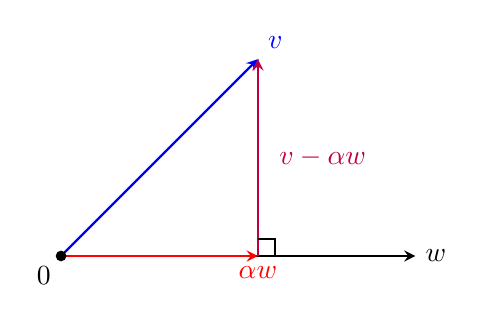
\begin{tikzpicture}[>=stealth, thick]
            % Оси / вектор w
            \draw[->] (0,0) -- (4.5,0) node[right] {$w$};

            % Вектор v
            \draw[->, blue] (0,0) -- (2.5, 2.5) node[above right] {$v$};

            % Проекция alpha*w
            \draw[->, red] (0,0) -- (2.5, 0) node[below] {$\alpha w$};

            % Перпендикуляр
            \draw[dashed, gray] (2.5, 2.5) -- (2.5, 0);

            % Обозначение v - alpha*w
            \draw[->, purple] (2.5, 0) -- (2.5, 2.5)
                node[midway, right=4pt] {$v - \alpha w$};

            % Значок прямого угла
            \draw (2.5, 0.22) -- (2.72, 0.22) -- (2.72, 0);

            % Точка начала координат
            \filldraw (0,0) circle (1.5pt) node[below left] {$0$};
        \end{tikzpicture}
    \end{center}
\end{definition}


\newpage

\begin{theorem}[об ортогонализации Грама-Шмидта]
    Пусть $v_1, \dots, v_m$ --- набор векторов в $V$. Тогда $\exists$ ортонормированный базис $e_1, \dots, e_k$
    линейной оболочки $\langle v_1,\dots, v_m\rangle$, такой что $\forall\, n \le k$ векторы $v_1, \dots, v_n \in \langle e_1, \dots, e_n\rangle$.
    \begin{proof}
        НУО $v_i \neq 0\ \forall\, i$. Индукция по $n$.\\[4pt]
        \textbf{База:} $n = 1$: $\quad e_1 \coloneqq \dfrac{v_1}{\|v_1\|}$\\[6pt]
        \textbf{Переход} $n \to n+1$:
        \[
            w_{n+1} \coloneqq v_{n+1} - \sum_{i=1}^{n} \langle v_{n+1}, e_i \rangle \cdot e_i
        \]
        Проверим ортогональность: $\forall\, j = 1,\dots,n$
        \[
            \langle w_{n+1}, e_j \rangle = \langle v_{n+1}, e_j \rangle - \langle v_{n+1}, e_j \rangle = 0
        \]
        \begin{center}
        \begin{tabular}{c|c}
            $w_{n+1} = 0$ & $w_{n+1} \neq 0$ \\[4pt]
            \hline\\[-6pt]
            $v_{n+1} \in \langle e_1, \dots, e_n \rangle$ & $w_{n+1} \perp e_1, \dots, e_n$ \\[6pt]
            & $e_{n+1} \coloneqq \dfrac{w_{n+1}}{\|w_{n+1}\|}$ \\[8pt]
        \end{tabular}
        \end{center}
    \end{proof}
\end{theorem}


\begin{stmt}
    Пусть $e_1, \dots, e_n$ --- ортогональный базис $V$. Тогда
    \[
        \forall\, v \in V \implies \exists\, \mathbf{\lambda}_1, \dots, \mathbf{\lambda}_n : \quad v = \sum_{i=1}
        ^{n} \mathbf{\lambda}_i e_i
    \]
    \[
        \langle v, e_k \rangle = \sum_{i=1}^{n} \mathbf{\lambda}_i \langle e_i, e_k \rangle = \mathbf{\lambda}
        _k \langle e_k, e_k \rangle
        \implies
        \boxed{\mathbf{\lambda}_k = \frac{\langle v, e_k \rangle}{\|e_k\|^2}}
    \]
    Если $e_1, \dots, e_n$ ортонормированы, то $\boxed{\mathbf{\lambda}_k = \langle v, e_k \rangle}$.
\end{stmt}


\begin{definition}
    Угол между векторами $v, w \in V$:
    \[
        \cos \angle(v, w) \coloneqq \frac{\langle v, w \rangle}{\|v\| \cdot \|w\|}
    \]
\end{definition}


\begin{definition}[Матрица Грама]
    Пусть $(v_1, \dots, v_n)$ и $(w_1, \dots, w_m)$ --- два набора векторов в $V$.
    Обозначим $\mathbf{v} = (v_1, \dots, v_n)$, $\mathbf{w} = (w_1, \dots, w_m)$. Тогда:
    \[
        \mathbf{v}^T \cdot \mathbf{w} =
        \begin{pmatrix}
            \langle v_1, w_1 \rangle & \langle v_1, w_2 \rangle & \cdots \\
            \langle v_2, w_1 \rangle & \ddots & \\
            \vdots & &
        \end{pmatrix}
        =: G_{\mathbf{v}, \mathbf{w}} \in \mathrm{Mat}_{n \times m}(\mathbb{R})
    \]
    Если $\mathbf{v} = \mathbf{w}$, то $G_{\mathbf{v}, \mathbf{v}} =: G_{\mathbf{v}} \in \mathrm{Mat}_{n \times n}(\mathbb{R})$.
\end{definition}

\newpage

\begin{stmt}
    Если наборы векторов $\mathbf{v}$ и $\mathbf{w}$ линейно выражаются через наборы
    $\mathbf{e} = (e_1, \dots, e_r)$ и $\mathbf{f} = (f_1, \dots, f_s)$
    по формулам $\mathbf{v} = \mathbf{e}\, C_{\mathbf{e}\mathbf{v}}$ и $\mathbf{w} = \mathbf{f}\, C_{\mathbf{f}\mathbf{w}}$,
    где $C_{\mathbf{e}\mathbf{v}} \in \mathrm{Mat}_{r \times n}(\mathbb{R})$ и $C_{\mathbf{f}\mathbf{w}} \in \mathrm{Mat}_{s \times m}(\mathbb{R})$, то:
    \[
        G_{\mathbf{v}\mathbf{w}}
        = \mathbf{v}^T \mathbf{w}
        = (\mathbf{e}\, C_{\mathbf{e}\mathbf{v}})^T\, \mathbf{f}\, C_{\mathbf{f}\mathbf{w}}
        = C_{\mathbf{e}\mathbf{v}}^T\, \mathbf{e}^T \mathbf{f}\, C_{\mathbf{f}\mathbf{w}}
        = C_{\mathbf{e}\mathbf{v}}^T\, G_{\mathbf{e}\mathbf{f}}\, C_{\mathbf{f}\mathbf{w}}
    \]
\end{stmt}


\begin{definition} [Определитель Грама]
    \[
    \Gamma_{\mathbf{v}} \coloneqq \det G_{\mathbf{v}}
    \]
\end{definition}

\begin{theorem}
    Для любого набора векторов $\mathbf{w} = (w_1, \dots, w_m)$:
    \begin{enumerate}
        \item $\Gamma_{\mathbf{w}} \ge 0$
        \item $\Gamma_{\mathbf{w}} = 0 \iff \mathbf{w}$ линейно зависим
    \end{enumerate}
    \begin{proof}
        Пусть $\exists$ ненулевой столбец $x = (x_1, \dots, x_m)^T \in \mathbb{R}^m$ такой, что
        \[
            \mathbf{w}x = x_1 w_1 + \dots + x_m w_m = 0
        \]
        Умножая слева на $\mathbf{w}^T$, получаем $G_{\mathbf{w}}x = 0$.
        Это означает, что строки (столбцы) матрицы $G_{\mathbf{w}}$ линейно зависимы, то есть матрица $G_{\mathbf{w}}$ вырождена, поэтому
        \[
            \Gamma_{\mathbf{w}} = \det G_{\mathbf{w}} = 0
        \]
        Если $w_1, \dots, w_m$ линейно независимы, то по т. Грама-Шмидта в их линейной оболочке $\exists$ ортонормированный базис
        $\mathbf{e} = (e_1, \dots, e_m)$. Тогда:
        \[
            G_{\mathbf{w}} = C_{\mathbf{e}\mathbf{w}}^T\, G_{\mathbf{e}}\, C_{\mathbf{e}\mathbf{w}} = C_{\mathbf{e}
            \mathbf{w}}^T C_{\mathbf{e}\mathbf{w}}
            \implies \Gamma_{\mathbf{w}} = (\det C_{\mathbf{e}\mathbf{w}})^2 > 0
        \]
        так как матрица перехода $C_{\mathbf{e}\mathbf{w}}$ обратима.
    \end{proof}
\end{theorem}



\begin{theorem}[Неравенство Коши–Буняковского–Шварца]
    Для любых $v, w \in V$:
    \[
        |\langle v, w \rangle| \le \|v\| \cdot \|w\|
    \]
    \begin{proof}
        Рассмотрим набор $\mathbf{v} = (v, w)$. По теореме об определителе Грама:
        \[
            \Gamma_{\mathbf{v}} = \det G_{\mathbf{v}}
            = \det \begin{pmatrix} \langle v,v\rangle & \langle v,w\rangle \\ \langle w,v\rangle & \langle w,
            w\rangle \end{pmatrix}
            = \langle v,v\rangle\langle w,w\rangle - \langle v,w\rangle^2 \ge 0
        \]
        Следовательно, $\langle v,w\rangle^2 \le \|v\|^2 \cdot \|w\|^2$, откуда $|\langle v,w\rangle| \le \|v\|\cdot\|w\|$.
    \end{proof}
\end{theorem}

\begin{examplelist}
    \item
    В $\mathbb{R}^n$ при $v = (x_1,\dots,x_n)^T$, $w = (y_1,\dots,y_n)^T$:
    \[
        \bigl(x_1^2 + \cdots + x_n^2\bigr)\bigl(y_1^2 + \cdots + y_n^2\bigr)
        \ge \bigl(x_1 y_1 + \cdots + x_n y_n\bigr)^2,
        \quad \forall\, x_i, y_i \in \mathbb{R}
    \]

    \item
    В $V = C([0,1])$ со скалярным произведением $\langle f,g\rangle = \int_0^1 fg\,dx$
    неравенство КБШ принимает вид:
    \[
        \int_0^1 f^2\,dx \cdot \int_0^1 g^2\,dx \ge \left(\int_0^1 fg\,dx\right)^2
    \]
\end{examplelist}

\begin{theorem}[Неравенство Гёльдера]
    Пусть $f, g \in C([0,1])$ и $p, q > 1$, $\dfrac{1}{p} + \dfrac{1}{q} = 1$. Тогда:
    \[
        \left(\int_0^1 f^p\,dx\right)^{1/p} \cdot \left(\int_0^1 g^q\,dx\right)^{1/q}
        \ge \left|\int_0^1 fg\,dx\right|
    \]
    \begin{remark}
        При $p = q = 2$ это в точности неравенство КБШ, и тогда
        $\left(\int_0^1 f^2\,dx\right)^{1/2} = \|f\|$ --- норма из скалярного произведения на $C([0,1])$.
        При произвольном $p \neq 2$ надо доказывать честно.
    \end{remark}
\end{theorem}
